%
% Template LaTeX for 3 pages report of TI2P2
%
\documentclass[reprint, a4paper, nofootinbib, amsmath, amssymb, aps]{revtex4-1}
% 
%
\usepackage[english]{babel}
\usepackage[utf8]{inputenc}
%\usepackage{graphicx}
\usepackage{bm}
\usepackage[breaklinks]{hyperref}
\usepackage{amsmath}
\usepackage{mathrsfs}
\usepackage{amssymb}
\usepackage{float}
\usepackage{comment}
\usepackage{hyperref}
%\usepackage{mathtools}
% \newcommand*{\bfrac}[2]{\genfrac{}{}{0pt}{}{#1}{#2}}
%\usepackage{epstopdf}
\usepackage[pdftex]{graphicx,color}
%\epstopdfDeclareGraphicsRule{.pdf}{png}{.png}{convert #1 \OutputFile}
%\AppendGraphicsExtensions{.pdf}
% \usepackage{pdfpages} 
% \usepackage{lipsum}

\usepackage{caption}
\usepackage{tikz}
\usetikzlibrary{calc}
\usepackage{feynmf}
\usepackage{xcolor}
%\usepackage{etex}
\usepackage{textcomp}
\usepackage{marvosym}
\usepackage{wasysym}
\usepackage{amsthm}
\usepackage{comment}
\usepackage{qtree}
\usepackage{tikz-feynman}
\usepackage{array}
\usepackage[yyyymmdd]{datetime}
\begin{document}

\title{Cheat Sheet for new Ph.D student in the CMS team of IPHC}

\author{a Former Ph.D student}
\affiliation{Université de Strasbourg, IPHC, 23 rue du Loess 67037 Strasbourg, France}

\date{\today}

\maketitle

%%%%%%%%%%%%%%%%%%%
\section{Introduction}

First and foremost, welcome to the CMS team of Strasbourg and congratulation for being promoted to Ph.D student (or intern). This paper will try to quickly give you tools and useful links to better understand what are all the acronyms that you may encounter, LaTeX related things, CMS related things, etc (Nothing related to the Ecole Doctoral will be mentioned as rules given may change over years...). This list won't be exhaustive as there are so many things to talk about but we hope that this will help you in any kind of way to fasten your progress in your work. For global IPHC commands, see: \href{https://twiki.cern.ch/twiki/bin/viewauth/CMS/IPHCusefulCommands#VScode}{IPHC useful commands}. There is also a nice VScode tutorial if you are not familiar with it, it's a nice looking and developed IDE. It can be possible that by the time of your Ph.D, ZED IDE became a thing or another one. Good luck!  

\section{Acronyms}
    A set of Acronyms is defined in a Twiki page in : \href{https://twiki.cern.ch/twiki/bin/view/CMSPublic/WorkBookGlossary}{TwikiAcronyms}. Twiki pages are like wiki pages but for the CMS documentation of everything. By the time you read this, this may have changed to gitlab or something else. We will just give some that you may encounter rapidly :
    \begin{itemize}
        \item POG : Physics object group : Muon POG, tau POG, EGamma POG, etc
        \item PAG : Physics Analysis Group : EXOTICA, Beyond-two-generations (B2G), TOP, etc
        \item L3-L2-L1 Conveners : Level 3 (2 and 1) conveners. There are responsible of a POG or PAG. And for example, the Long-lived Particle (LLP) group is a level-3 PAG below the Level-2 : Exotica. See the twiki page of LLP \href{https://twiki.cern.ch/twiki/bin/viewauth/CMS/ExoticaLongLived}{TwikiLLP}.
        \item CADI-line : Reference number for any analysis : EXO-19-001, B2G-22-005, HIG-22-004
        \item AN : Analysis Note : every details of an Analysis written in paper (restricted access to people from the collaboration)
        \item PAS: Physics Analysis Summary : Summary of an Analysis Note, basically
    \end{itemize}
%%%%%%%%%%%%%%%%%%%
\section{Compact Muon Solenoid detector }
    
    %----------------%
    \subsection{Point 5}

    The CMS detector is situated at one of the crossing point between the two beams of the LHC, also called Point 5 or P5. During your Ph.D, you will have to perform shift at P5 (trigger shifts, Data Quality Monitoring (DQM), Shift Leader, Data Acquisition System (DAQ), DCS Detector Control Status). There are different types of shifts, online (usually at P5) and offline (can be performed outside of P5 usually). A shift last 8 hours where you take care of one aspect of the detector mentioned above and have to communicate important information to others, the shift leader especially.
    It may change over time but a certain amount of shifts have to be performed by the CMS team of IPHC (there are quotas) and usually online shifts are the ones that are done to fulfill the quotas (even more points when doing night shifts). All the links related to the different shifts will not be given here as they may be updated quite often and are really specific. No worries, everything will be given to you by shifts coordinators when the time will come. \\
    Personal Experience: Trigger Shifts and DQM shifts are pretty cool and all kinds of shift help you better understand the experiment
    
    PS: Becareful, P5 is NOT on the Meyrin or the Prevessin sites. You need to take your car or the shuttle to get to P5 as CMS is wondering around in the countryside. There is also the car-sharing system of CMS. Taking the bike is not really recommended.
    


    \subsection{The detector}
    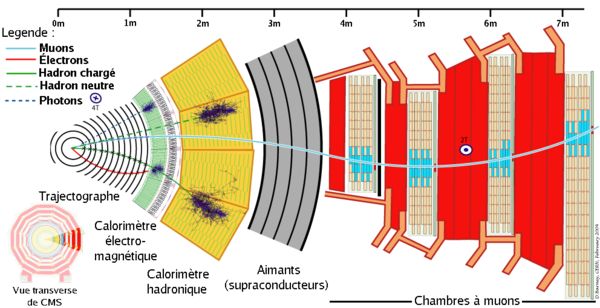
\includegraphics[height=4cm, width=8cm, trim= 0cm 0cm 0cm 0cm,clip]{Images/cmsAll.png}
    \captionof{figure}{Transverse view of CMS}
    \label{fig: CMS}
    The CMS detector is 15 meter wide and 21 meter long. You can see a transverse view of CMS in Fig.\ref{fig: CMS}. The description will be a bit biased since the Strasbourg team is highly involved in the current tracker and its upgrade. At the very center, the closes part with respect to the interaction point is the beam pipe.Then comes the tracker that is divided into two parts (see Fig.\ref{fig: Tracker}) : Pixels and strips. Pixels are the innermost part of the tracker and also divided in to two parts: Barrel Pixels (BPIX) and Forward Pixels (FPIX). After the Pixels are the strips also divided into several parts: Tracker Inner Barrel (TIB), Tracker Outer Barrel (TOB). Then, there the two forward parts : the Tracker Inner Disks (TID) and Tracker End Caps (TEC). The characteristics (pitch, width, etc) of the modules of the silicon strip tracker change depending on where there are in the tracker.
    For the tracking, an iterative process is implemented to look for tracks. For electrons, it's slightly different due to Bremsstrahlung, the tracking is using the GaussianSum filter to take into account the information of photons. You may therefore encounter GSF electrons when coding :D. THe goal of the tracker is to reconstruct the tracks of charged particles (that deposits energy in the layers of the tracker)\\
    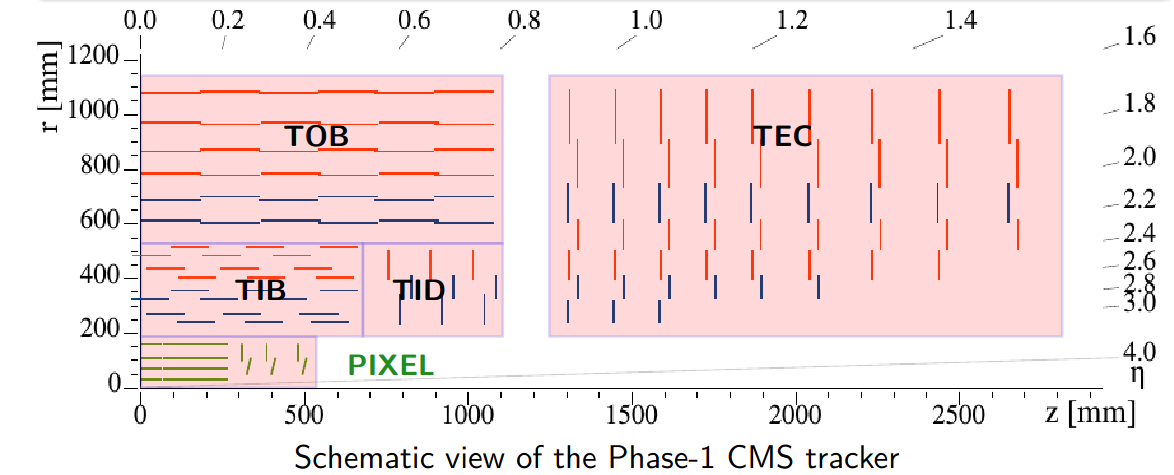
\includegraphics[height=4cm, width=8cm, trim= 0cm 0cm 0cm 0cm,clip]{Images/CMSTracker.png}\label{fig: Tracker}
    \captionof{figure}{Phase-I tracker of CMS (Phase-0 Tracker had one less FPIX and BPIX layer + slightly different positions  for the Pixel layers)}
    After the tracker comes the Electromagnetic and hadronic calorimeters. The former is used to detect energy deposits from photons and electrons (used for the GSF tracking). The hadronic calorimeter is used to detect energy deposits from both neutral and charged hadrons. \\
    Finally, there are the muons chambers. Again there are different types of subdetector for muon chambers like Resistive Plate Chambers (RPCs), Cathode Strip Chambers (CSC), Gas Electron Multiplier (GEM), Drift Tubes (DTs).Here is a small document to explain how each one of them works : \href{https://cds.cern.ch/record/2698492/files/Poster-2019-989.pdf}{Muon Poster} (click on Muon Poster).

    Since you are working in the Strasbourg team, some part of your work may be related to the tracker, here are a few links to better understand the tracker :
    \begin{itemize}
        \item \href{https://indico.cern.ch/event/1238081/timetable/#20230227}{Tracker training days 2023} : a lot of slides about everything concerning pixels and strips
        \item If you like reading more than going through slides, here is \href{https://cds.cern.ch/record/914891/files/jpconf6_41_011.pdf}{Doc Tracker}. Quite old but gives the basics
        \item Quantities related to the tracker : \href{http://cms.cern.ch/iCMS/jsp/openfile.jsp?type=DN&year=2020&files=DN2020_004.pdf}{Click}
    \end{itemize}
    
%%%%%%%%%%%%%%%%%%%
\section{LaTeX}
    You might need to use some LaTeX during your Ph.D, only examples will be given and a cheat sheet (all the examples are given as zip files that you can open in overleaf or you ;can just check the code):
    \begin{itemize}
        \item \href{https://wch.github.io/latexsheet/}{Cheat Sheet}
        \item FeynMan Diagrams : examples are given in the twiki page, see ppToXX 
        \item Poster : an exemple is given : Poster CMS Week ...
        \item Of course, there are many more things to know but this will give you the basics if you are a beginner
    \end{itemize}

    You will see that the TikZ library is used and is kinda common to draw shapes, add things to already existing plots, Feynman diagrams, etc. When using the tikzFeynman library or tikz in general, you may need to change the compiler of overleaf to lualatex in the Menu on the top left.
    
\section{root}

 Only few things will be given as there are not much things to know  about ROOT.
 Be always careful about the version of root you are using as you may face root version incompatibility. You can change the version of root you are using by doing this command  on the uiX: \\
 \begin{center}
     $\rightarrow$ ls  /libcern/root (to check which version are available) \\
     $\rightarrow$ source /libcern/root/6.24.06/centos7.6-x86\_64/bin/thisroot.sh to change of version (for example)
 \end{center}

    From a root Ntuple where you have stored branches, you can open the file in a TBrowser and do :
    \begin{center}
        "name of the tree"-$>$MakeClass("toto")
    \end{center}
  It will create a .c and .h file that you can use directly to run over the events of the ntuple.\\
  Again, with a Ntuple, you can use the edmDumpEventContent $<$name of file$>$ to check the collections available in the file
  
  Another point that can be really useful if you are running on Ntuples and you know that it will take quite some time to produce the output file (usually a root file with some histograms) : RDataframe. It is quite recent but different from basic c++. However, it is really powerful when you are applying basic  selections to produce histograms as it is performing columnar operations and not looping over events. It is also powerful as you can activate multi-threading allowing to run on multiple cpu's fastening your code. For example, in m case, a 5-hour long code took 3 min :D. An exemple of RDataframe code is given in the directory RDataFrame. 
\section{Physics Analysis}

    When you start a physics analysis, you will probably invited to look for a Beyond the Standard Model physics process or improve a measurement of an existing quantity. For the former, since what you are looking for has not yet been discovered, you need simulation to learn the behavior of your signal in the CMS experiment. To simulate events (we say Monte-Carlo events or MC events), you need a generator. The one that you may encounter the most is MadGraph and you can actually use it on your own if you want (See Tutorial\_MC\_production\_for...). MadGraph is usually combined with another one, it can be Pythia8, powheg (there are others) to take care of the hadronisation as madgraph is not really efficient with the simulation of low energy jets while the other two have a better description of the low energy jets.  This is why you will encounter the name of Madgrapg and pythia or powheg when looking at MC samples in the CMS database (\href{https://cmsweb.cern.ch/das/}{CDAS}). Here are a few examples :\begin{itemize}
        \item /TTTo2L2Nu\_TuneCP5\_13TeV-powheg-pythia8
        \item /ST\_tW\_top\_5f\_NoFullyHadronicDecays\_TuneCP5\_13TeV-powheg-pythia8
        \item /TTWW\_TuneCP5\_13TeV-madgraph-pythia8
    \end{itemize}
    The first bullet is a $t\Bar{t}$ sample where both W coming from the top decays decay leptonically. The TuneCP5 is a set of parameter of the generators. There can be many names for the tunes but CP5 is a common one. The final output of the generator is a LHE file (Les Houches Event file). It contains all the information related to the event generated (4-vectors, lifetime, mass, pdf weights, etc). The generation part of the events is done outside/independent of the CMS environment (but you have to take into account some CMS parameters like the PDF of the energy of the beams, etc).

    Now, the CMS process will come into place. There are 4 steps to follow in order to generate the events that you will be able to analyze.    
    We won't go into details but the command that is used is here \href{https://twiki.cern.ch/twiki/bin/view/CMSPublic/SWGuideCmsDriver}{CMSDRIVER}. If you have to use this command, you may ask the MC\&I contact of your PAG for help. The final output is a root file that contains a certain amount of information. This "amount" will depend on the data format that you want to use : RAW, RECO, AOD, MniAOD, Nanoaod (see : \href{https://twiki.cern.ch/twiki/bin/view/CMSPublic/WorkBookAnalysisOverviewIntroduction}{DataFormats}). 
 
    CMS is actually pushing towards NanoAOD but RECO, AOD and MiniAOD can still be used. For your analysis, there is a high chance that you work with at least AOD if not MiniAOD if not nanoAOD :D. \\
    Depending on the data format that you are using, the collection of physics object (codewise) that you can use is different. Links are provided in the \textbf{Physics Object} section.\\

    A global overview of an analysis is given in this workbook \href{https://twiki.cern.ch/twiki/bin/view/CMSPublic/WorkBook}{Analysis Workbook}\\
        
    
\subsection{Analysis Strategy}
    Once you have decided of the physics process you want to observe (and generated the MC samples of your signal if needed), you will have to define a set of cuts to observe your signal as it may be hidden because of too much background. These cuts can be performed on some basic kinematic variables but they can be much more sophisticated using Machine learning (Graph Neural Network, Boosted Decision Tree, Convolutionnal Neural Network, etc.). Most cuts have to keep the maximum of signal events while removing as much as possible the background events. First, you have to test the cuts on some MC samples (signal and background). Once you are satisfied with your cuts on simulation, you can go to the data (be careful, do not look at the signal region, where you expect to observe your signal as it is forbidden, you need the agreement of the CMS collaboration). To define a signal region, you will sometimes hear about the ABCD method which is about separating the phase space into 4 regions : A,B,C and D. For that, you need two decorrelated variables that you apply a cut on.
    We won't go further than that but the thing to remember is to define what you want to observe at the end: a mass, an angle, a specific distribution, etc. and how you define your region of signal, with which sets of cuts.\\
    \textbf{Note 1 :} If you are using private MC samples for your analysis, try to get a central production of them as soon as possible, it will avoid some unnecessary stress at the end of your Ph.D. You should discuss with the MC\&I contact of your group but you can already have a look at this : \href{https://cms-pdmv.gitbook.io/project/mccontact#preliminary-steps}{Steps to follow} and also this : \href{https://twiki.cern.ch/twiki/bin/viewauth/CMS/GitRepositoryForGenProduction}{generate pull request}.
    \textcolor{red}{\textbf{Note 2:}} From all the configuration tested, only one works (the one that is not recommended :D \dots) : in cmssw-el7 singularity, you need to run the gridpack generation command with those parameters : ./gridpack\_generation.sh "name" cards/"name"/ local ALL slc7\_amd64\_gcc10 where "name" is the name of your process of your MG5 cards. And sorry, I can't really help with the fragments, I never quite understood how they worked. The only thing I can tell is to start with basic fragments and may be discuss with the MC&I contact. (example of fragment : genFragments/Hadronizer/13TeV/Hadronizer\_TuneCP5\_13TeV\_MLM\_5f\_max1j\_LHE\_pythia8\_cff.py)
    
\subsection{Run 2}
    Global information about Run 2 : \\
    \href{https://twiki.cern.ch/twiki/bin/view/CMS/PdmVRun2LegacyAnalysis}{Global Information} \\
    \href{https://twiki.cern.ch/twiki/bin/viewauth/CMS/PdmVAnalysisSummaryTable}{Summary of what to use} \\
    Then, the MC simulation may not represent the data because data is hard to reproduce correctly. There can be detector effect to be taken into account. All these things need corrections that can be found in the following links : 
    \href{https://twiki.cern.ch/twiki/bin/view/CMS/PileupJetIDUL#Recommendations_for_2018_UL_data}{PileUp reweighting info} \\
    \href{https://twiki.cern.ch/twiki/bin/view/CMS/LumiRecommendationsRun2}{LumiREcommendations} \\
    \href{https://twiki.cern.ch/twiki/bin/view/CMSPublic/WorkBookJetEnergyResolution}{Jet Energy resolution} \\
    \href{https://indico.cern.ch/event/1247210/sessions/478562/attachments/2587866/4465075/MuonPOG_tutorial_part2.pdf}{MuonSF} \\
    \href{https://twiki.cern.ch/twiki/bin/viewauth/CMS/SWGuideMuonIdRun2}{MuonID} \\
    \href{https://twiki.cern.ch/twiki/bin/view/CMS/RochcorMuon}{RochesterCorrections}\\
    There are many more things to know but this give you a firstview of what to check. You can also check the page that summarizes kind of everything : \href{https://twiki.cern.ch/twiki/bin/view/CMS/TopSystematics}{TopSyst} 
    
\subsection{Run 3}
    Global information about Run 3 : \href{https://twiki.cern.ch/twiki/bin/view/CMS/PdmVRun3Analysis#Run_3_Analysis}{Click}

    You can follow the links for Run 2, there may redirect you to Run 3 pages :D or still be valid for Run 3.
\subsection{Physics Object}
    It may be useful when you are starting an analysis from scratch. If you are using an already existing framework for your analysis, then you might not care about the following. \\
    For the different data format, you do not manipulate the physics object in the same way, so here are two workbooks for the MiniAOD and NanoAOD : \\
    \href{https://twiki.cern.ch/twiki/bin/view/CMSPublic/WorkBookMiniAOD2017}{MiniAOD}\\
    \href{https://twiki.cern.ch/twiki/bin/view/CMSPublic/WorkBookNanoAOD}{NanoAOD}\\
    Yeah, we know it is from Run 2, welcome to CMS where nothing is really up-to-date.



\subsection{Combine}


    Once you have implemented your analysis strategy, you need to set limits on some cross-sections, couplings, masses, or even define scale factors. A tool has been developed within the CMS collaboration and made available to anyone : \href{https://cms-analysis.github.io/HiggsAnalysis-CombinedLimit/latest/}{Combine}. It was first used to discover the Higgs boson back in 2012. Now, it  has a general purpose and really powerful. However, it takes quite some time to fully grasp and understand everything. Following the tutorial first is the best (and a decent understanding of statistics is needed)- \href{https://cms-analysis.github.io/HiggsAnalysis-CombinedLimit/latest/part5/longexercise/}{Tutorial}. You will probably see some Brazilian plots in your time here, and they may come from Combine.

\section{crab}

 During your Ph.D, you may need to run on MC simulation samples with millions of events. You can do that on your local computer but you may finish your Ph.D  before you finish analyzing the events. To address this issue, you have access to a grid. For that, you need a certificate that needs to be updated once every year. \href{https://twiki.cern.ch/twiki/bin/view/CMSPublic/WorkBookChapter5}{CMSCertificate} and \href{https://indico.in2p3.fr/event/32895/}{Yannick's slides}. Once you have your certificate, you can submit crab jobs using the following commands (in a cms environment area): 
 
'source /cvmfs/cms.cern.ch/crab3/crab.sh' \\
'voms-proxy-init -rfc -voms cms -valid 192:00'\\
'crab submit -c crab\_config\_mc\_2018.py' \\

where crab\_config\_mc\_2018.py is a configuration file for your crab jobs. A version of config file is given in the git repository (multicrab) that allows to launch on multiple  MC sample.

You have to use slightly different commands for that :
./multicrab --crabCmd submit (to launch the jobs)

./multicrab --crabCmd status --workArea ./$<$work\_directory$>$ (to get the status of the jobs : failed, idle, running, finished or not submitted)\\
./multicrab --crabCmd kill --workArea ./$<$work\_directory$>$ (to kill the jobs )\\
./multicrab --crabCmd resubmit --workArea ./$<$work\_directory$>$ (resubmit failed jobs)\\

To get the outpule files, you need to use the gfal commands :
(You have to do that without setting the cmsenv but only :\\
source /cvmfs/cms.cern.ch/crab3/crab.sh )\\
gfal-ls davs://sbgdcache.in2p3.fr/cms/phedex/store/user/$<$Your directory$>$\\
gfal-copy -r davs://sbgdcache.in2p3.fr/cms/phedex/store/user/$<$Your directory$>$ \\
Then you will probably need to hadd (gather together) the different output files and you are done.
Here is the documentation of the crab config file : \\
\href{https://twiki.cern.ch/twiki/bin/view/CMSPublic/CRAB3ConfigurationFile}{CrabconfigFile}

\section{Remote working/ background tasks}

During your Ph.D/ internship, you may want to run programs while you are enjoying life or your code takes multiple hours to finish (even days) and you don't want to keep your computer open. Depending on the servers you are logged in, the solution is different :

\begin{itemize}
    \item uiX \begin{enumerate}
        \item screen -S $<name>$
        \item  "crtl+a+d" to detach from the session
        \item screen -R (to view all the sessions you have opened)
        \item screen -R $<name>$ (to continue working on a session)
        \item screen -X -S $<name>$ to kill a session
    \end{enumerate}
    \item lxplus \begin{enumerate}
        \item systemctl --user enable --now tmux.service (only the first time, i think)
        \item tmux new -s $<name>$
        \item "crtl+b"+d to detach from the session ("exit" if you want to kill the session)
        \item tmux ls (to view all the sessions you have opened)
        \item tmux attach -t $<name>$ (to continue working on a session)
    \end{enumerate}
\end{itemize}
%%%%%%%%%%%%%%%%%%%
\section{Storage of data at IPHC}
For the people using crab (and potentially other systems), the output will be stored on dcache. To access the your data, you will need to have a valid certificate and enter the following command (NOT IN A cms environment):\begin{itemize}
    \item source /cvmfs/cms.cern.ch/crab3/crab.sh 
    \item (Potentially :) voms-proxy-init -rfc -voms cms -valid 192:00
    \item gfal-ls davs://sbgdcache.in2p3.fr/cms/phedex/store/user/$<name>$ to list the files (no option for ls is available)
    \item Example : gfal-ls davs://sbgdcache.in2p3.fr/cms/phedex/store/user/pvaucell/
    \item gfal-copy -r davs://sbgdcache.in2p3.fr/cms/phedex/store/user/pvaucell/$<directory>$ . to copy files
\end{itemize}
\section{Conclusion}

I hope that it somehow helped you. It is not exhaustive and probably not up-to-date when you will be reading it but it gives hints or potential solution to your issues. Good luck in your Ph.D (or internship).\\
PS : Any feedback is appreciated ! (paul.vaucelle@iphc.cnrs.fr up until september 2025, after that i don't know )

La Relève 
%%%%%%%%%%%%%%%%%%%%%%%%%%%%%%

\end{document}
